\section{Introduction}
Matched-field processing is a popular used method in underwater acoustics and requires a pretty good knowledge of environment, thus it is sensitive to the model mismatch and performs poorly in unstable and complicated ocean environments.
While, machine learning based methods can perform a required calculation through learning form examples directly and do not require a good a priori information.
A notable recent example of using machine learning method in underwater acoustic is the application of nonlinear classification to source localization\cite{niu2017source}.
Niu assumes there existing a deterministic relationship between ship range and sample-covriance matrix and approximated this relationship by the feed-forward neural networks(FNN).
The algorithm performs well on the Noise09 experimental data, which suggests that FNN can achieve a good prediction performace if source localization is solved as a classification problem.
In Niu's work, the neural networks used is dense and the trained model is also sensitive to the mismatch problem. Dense neural networks can learn a over-complete
representation of input data but need much storage and computation.

In this paper, based on Niu's work, we train the feed-forward neural networks with sparse constraint and use data-model mixed training to improve the model tolerance. Our algorithm was tested on SWell96 experimental and simulated data.


\section{Neural Networks Based Source Localization}
In this section, we discuss how to establish a source localization prediction model using neural Networks and how to learn parameters in the model.

\subsection{Neural Networks Models and Function Approximation}
As we known, neural networks models can be viewed as a mathematical function $f$. Taking feedforward neural network(FNN) as an example, it defines a mapping ${{y}}=f(x;\theta )$ between input $x$ and output $y$ by parameter $\theta$, which needed to be learned by a rule. Feedforward networks are called networks because they are typically represented by composing together many different functions. We might have two function $f^{1}$, $f^{2}$ connected in a chain\cite{goodfellow2016deep}, to form
$f(x) = f^{2}(f^{1}(x))$.

FNN extend linear models to represent nonlinear transformed format $\phi(x)$ of input $x$. The transform function $\phi$ can be thinked as providing a set of features describing $x$, or as providing a new representation for x. The key problem here is how to choose the mapping $\phi$.

The strategy of machine learning is to learn $\phi$. In a feedforward network, $\phi$ defines a hidden layer $h=\phi(x;w^{(1)})$, then the total model is $y=f(x;\theta)=hw^{(2)}$.
Obviously, we need to learn $\phi$ from a broad class of functions, and parameters $w$ mapping $\phi(x)$ to the desired output.

In most cases, our parametric model defines a distribution $p(y|x;\theta)$. Simply, we can use the principle of maximum likelihood to learn parameters in model.
\begin{equation}
J(\theta ) =  - {E_{x,y \sim {p_{data}}}}\log {p_{model}}(y|x)
\end{equation}
where the specific form of $p_{model}$ is defined by networks.
As maximum likelihood is a consistent estimator, the model is capable of representing the training distribution.

\subsection{Regularization for neural networks}

There are two main kind of regularization strategies for neural networks, one is weight-level regularization, another is neuron-level regularization with activation penalty.
\begin{equation}
\tilde J(\theta ;X,y) = J(\theta ;X,y) + \alpha \Omega (\theta )+ \beta \Omega (h)
\end{equation}
where $\Omega (\theta )$ is parameter norm penalty, $\Omega (h)$ is penalty on the activations of the units, $\alpha$,$\beta$ are hyper parameters that weight the relative contribution of
the norm penalty term. Weight decay term penalize the size of the model parameters, while, the activation penalty term encouraging their activations to be sparse.

\subsection{Training the neural networks with sparse constraint}
In practical applications, we not only want the representation to be sparse, but also want the model features to be sparse, the latter saves the storage and calculation on sensor nodes. Thus, we use $L1$ norm to promote sparse neurons activations, and constrain the norm of each column of the weight matrix to prevent any one hidden unit from having very large weights.
\begin{equation}
\begin{split}
&\tilde J(\theta ){\kern 1pt} {\kern 1pt} {\kern 1pt} {\rm{ = }}{\kern 1pt} {\kern 1pt} {\kern 1pt}  - {E_{x,y \sim {p_{data}}}}\log {p_{model}}(y|x){\rm{ + }}{\kern 1pt} {\kern 1pt} \lambda {\left\| h \right\|_1}\\
& s.t.{\kern 1pt} {\kern 1pt} {\kern 1pt} {\kern 1pt} {\kern 1pt} {\kern 1pt} {\kern 1pt} {\kern 1pt} {\kern 1pt} {\kern 1pt} {\left\| {{W^{(1)}_i}} \right\|_2} \le C{\kern 1pt} {\kern 1pt} {\kern 1pt} {\kern 1pt} {\kern 1pt} {\kern 1pt} {\kern 1pt} {\kern 1pt} {\kern 1pt} \forall {\kern 1pt} i = 1, \cdots ,M\\
\end{split}
\end{equation}
In the equation, $M$ is the number of neurons in hidden layer.
When a useful sparse representation of any given data is learned, each datum will then be encoded as a sparse code, thus we can use the least possible amount of resource to store or transfer the data.

What we need to do here is learning a set of basis functions $\phi(x)$ that make the given data can be represented sparsely.
As the neuron networks do, we use a linear model with nonlinear function to fit the basis functions.
\begin{equation}
h = g(W^{(1)}x + b^{(1)})
\end{equation}
Activations between hidden layer and output layer are connected by a linear combinations:
\begin{equation}
z = {W^{(2)T}}h + {b^{(2)}}
\end{equation}
The output of the model is normalized by $softmax$ function, which is a common choice for multi-class classification task\cite{bishop2006pattern}:
\begin{equation}
p({y_k}|x) = softmax {(z)_k} = {{\exp ({z_k})} \over {\sum\nolimits_j {\exp ({z_j})} }}
\end{equation}
where $g$ is the nonlinear function, $h$ is the the desired the sparse data, $x$ is the measures, $p({y_k}|x)$ is the probability measured signal $x$ trasmitted from position $k$, $W$ and $b$ is the parameters needed to learned.

% \subsection{Source localization prediction}
% After the model parameters learned in section 2.3, the position distribution probability $y$ can be predicted for an unlabled data, the position label is mapped to the source localization.
% \begin{equation}
% position = \mathop {argmax}\limits_k p({y_k}|x)
% \end{equation}
% Source position is 

\section{Simulation and experimental results}
In this section, same as Niu's work\cite{niu2017source}, we implement a simple FNN with just one hidden layer to learn source range directly from SWellEx96 acoustic data, and compare the performance of the classifier with the conventional matched-field processing method (Bartlett) in terms of simulation data and experimental data, respectively. In addition, the influence of sound speed profile(ssp) mismatch on the performance of FNN classifier is investigated by simulations. We improve the tolerance of the classifier by training the model using data sampled under different ssp.

Simulation environment is the widely studied SWell96Ex test, conducting in a 216m deep shallow waveguide environment. 
During the experiment, the source ship has two sound source, a deep source (J-15) and a shallow source (J-13). In all the simulations, we used the shallow sound source, which was towed at a depth of about 9m and transmitted 9 frequencies between 109Hz and 385Hz.

\subsection{Parameter settings}
In simulation part, acoustic data used to train and test the neural network is simulated using kraken with environment model.  We also use the normalized sample-covariance matrices of measured pressure at each frequency as model input data. In input layer, number of neurons $D$ is $L^{2} \times N_{fre}$(number of frequency used). The number of neurons in the output layer (number of classes) $K = 300$. Simply, we set the number of neurons in hidden layer equal to the input layer, i.e. $M = D$. Fast	Fourier	transform duration is 1-seconds, Snapshot $N_{s}$ for constructing SCMs is 10. The number of vertical array elements $L$ is 21. Specifically, the cost function now becomes

%\begin{equation}
%\begin{split}
%&\min {\kern 1pt} {\kern 1pt} {\kern 1pt} {\kern 1pt} {\kern 1pt} {\kern 1pt} \tilde J(\theta ){\kern 1pt} {\kern 1pt} {\kern 1pt} {\rm{ = }}{\kern 1pt} {\kern 1pt} {\kern 1pt} {\rm{ - }}{{\rm{1}} \over N}\sum\limits_{n = 1}^N {\sum\limits_{k = 1}^K {{t_{nk}}\ln {y_{nk}}{\kern 1pt} {\kern 1pt} {\kern 1pt} {\rm{ + }}{\kern 1pt} {\kern 1pt} \lambda {{\left\| h \right\|}_1}} }\\
%& s.t.{\kern 1pt} {\kern 1pt} {\kern 1pt} {\kern 1pt} {\kern 1pt} {\kern 1pt} {\kern 1pt} {\kern 1pt} {\kern 1pt} {\kern 1pt} {\left\| {{W_i}^{(1)}} \right\|_2} \le C{\kern 1pt} {\kern 1pt} {\kern 1pt} {\kern 1pt} {\kern 1pt} {\kern 1pt} {\kern 1pt} {\kern 1pt} {\kern 1pt} \forall {\kern 1pt} i = 1, \cdots ,M\\
%\end{split}
%\end{equation}
\begin{equation}
{\kern 1pt} {\kern 1pt} {\kern 1pt} {\kern 1pt} {\kern 1pt} {\kern 1pt} \tilde J(\theta ){\kern 1pt} {\kern 1pt} {\kern 1pt} {\rm{ = }}{\kern 1pt} {\kern 1pt} {\kern 1pt} {\rm{ - }}{{\rm{1}} \over N}\sum\limits_{n = 1}^N {\sum\limits_{k = 1}^K {{t_{nk}}\ln {y_{nk}}{\kern 1pt} {\kern 1pt} {\kern 1pt} {\rm{ + }}{\kern 1pt} {\kern 1pt} \lambda {{\left\| h \right\|}_1}} }
\end{equation}
where $t_{nk}$ and $y_{nk}$ are real and predictive probability of sample data $x$ belongs to class $k$ separately. We choose $C=1$ here.
For the sake of learning speed and sparsity of hidden neurons, we use the $ReLU$ activation in hidden layer.
The training set is 3000 samples of uniform sampling between 1.82\--8.65km, test set is another 300 data samples sampling from the same range. The noise in the simulations is all set to be complex gaussian white noise.

\begin{figure}
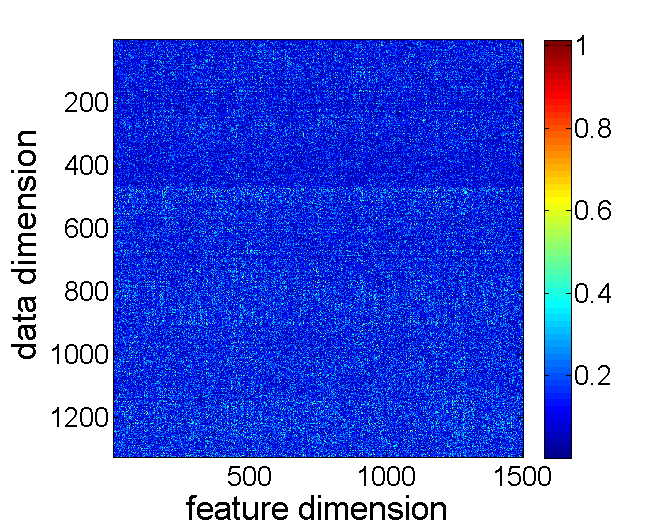
\includegraphics[width=4cm,height=3cm]{figure/Weights_summaries_in_hidden_laye_swell_exp}
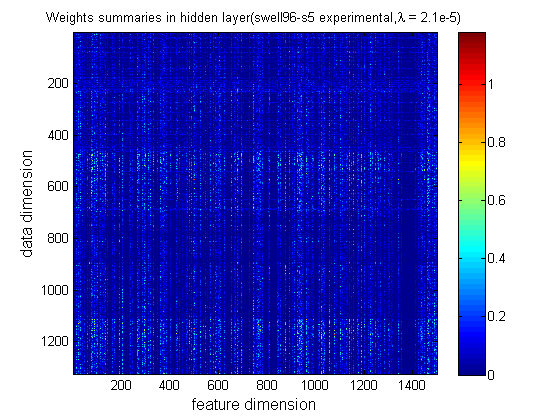
\includegraphics[width=4cm,height=3cm]{figure/Weights_summaries_in_hidden_layer_swell_exp_lambda_2_dot_1e_neg_5}
%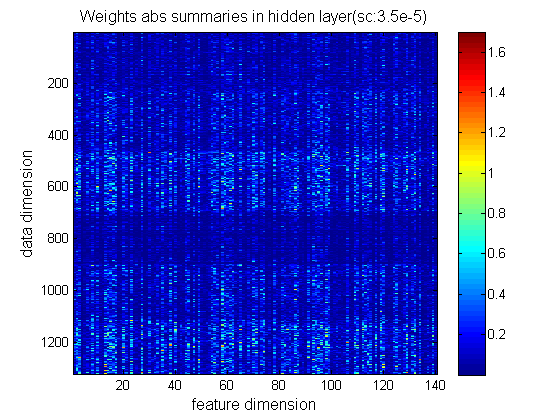
\includegraphics[width=4cm,height=3cm]{figure/Weights_abs_summaries_in_hidden_layer_sc3dot5e_nag_5_swell_140}
%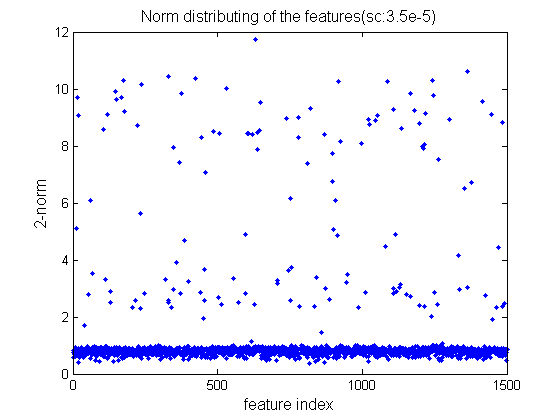
\includegraphics[width=4cm,height=3cm]{figure/Norm_distributing_of_the_features_sc3dot5e_nag_5_swell}
\caption{Weights summaries in hidden layer(left:no constraint,right:with constraint). sparse constraint
training makes the weight coefficient show the group structure,either all zero,or basic is not zero.}
\end{figure}

Experimental data gets from SWell96Ex Event S5 vertical line array(VLA) . The array recorded a total of 75 min of data. In order to facilitate processing, we took 0\--50min data as a training set.

Consistent with the simulation part, we divide the trajectory into 300 grids, 25m each. We set 1-second as a snapshot and get 3000 sample-covariance matrixs (SCMs), the sample-covariance matrix is averaged at every two snapshots.
At the time of training, we took 9/10(2700)of samples as training set and another 1/10(300) as test set.

\subsection{The effect of sparse constraint training}
The regularization degree on model affects the model error and average activation density of FNN's hidden layer. As the coefficient grows, the model error on training set and test set also grows, but slower on test set, which means
the regularization helps improving the performance on test data in some sense. The model error is defined as the dissimilarity between true probability distribution and estimated probability distribution, thus the Kullback-Leibler(KL) divergence.
In Fig.2, we use the cross entropy equivalently.

On the other hand, the regularization on neuron-level significantly reduces the average activation density,
The order of magnitude drops from $10^{3}$ to $10$, and keep it stably. This phenomenon is a good news for
us to train a sparsely-coded neural networks.

Compared to the case of training without sparse constraints, sparse constraint makes the weight coefficient in the hidden layer show the group structure, either all zero, or basic is not zero. Take the case $\lambda=2.1 \times 10^{-5} $
for example, the number of feature vectors reduced from 1500 to 740, as shown in Fig.1. In addition, it can be seen that the relative size of learned weights is related to the frequency, and even at the same frequency, the the weight corresponding
to real and imaginary parts is also different, we can see bright and dark strip distribute along the data dimension in Fig.1. The data dimension is arranged according to the frequency relationship when we plot the weights summaries in Fig.1.

\begin{figure}
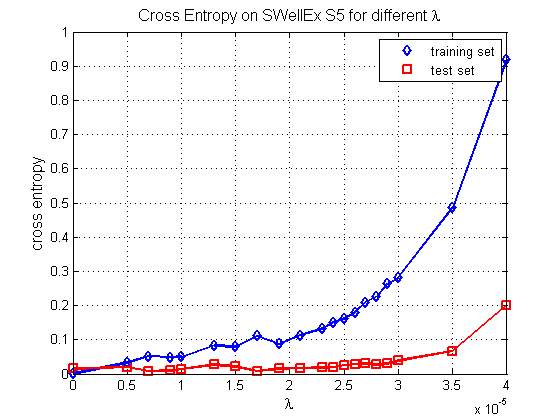
\includegraphics[width=4cm,height=3cm]{figure/Cross_Entropy_on_SWellEx_S5_for_different_lambda}
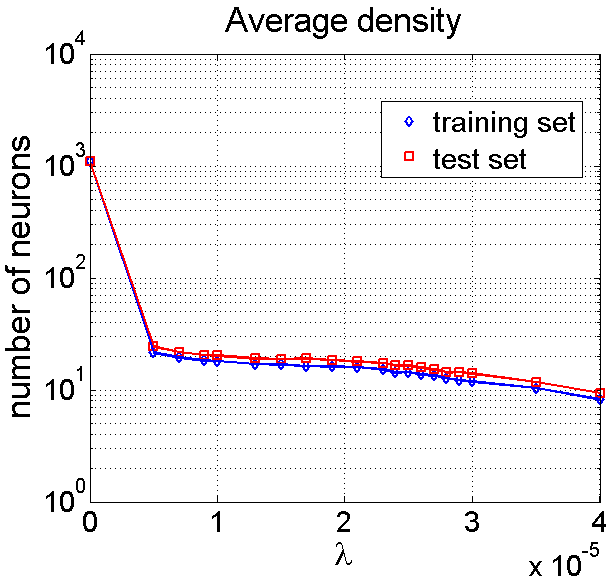
\includegraphics[width=4cm,height=3cm]{figure/Hidden_Average_Density_on_SWellEx_S5_for_different_lambda}
\caption{Model error and Average-activation-density for different $\lambda $.  Regularization on neuron-level
significantly reduces the average activation density without much cost in model error.}
\end{figure}


%\begin{figure}
%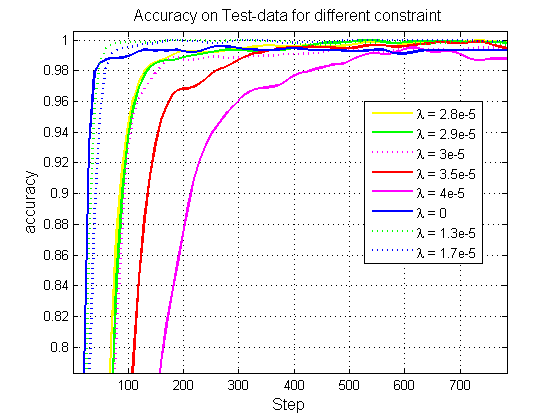
\includegraphics[width=4cm,height=3cm]{figure/Accuracy_on_Test_data_for_different_constraint_exp}
%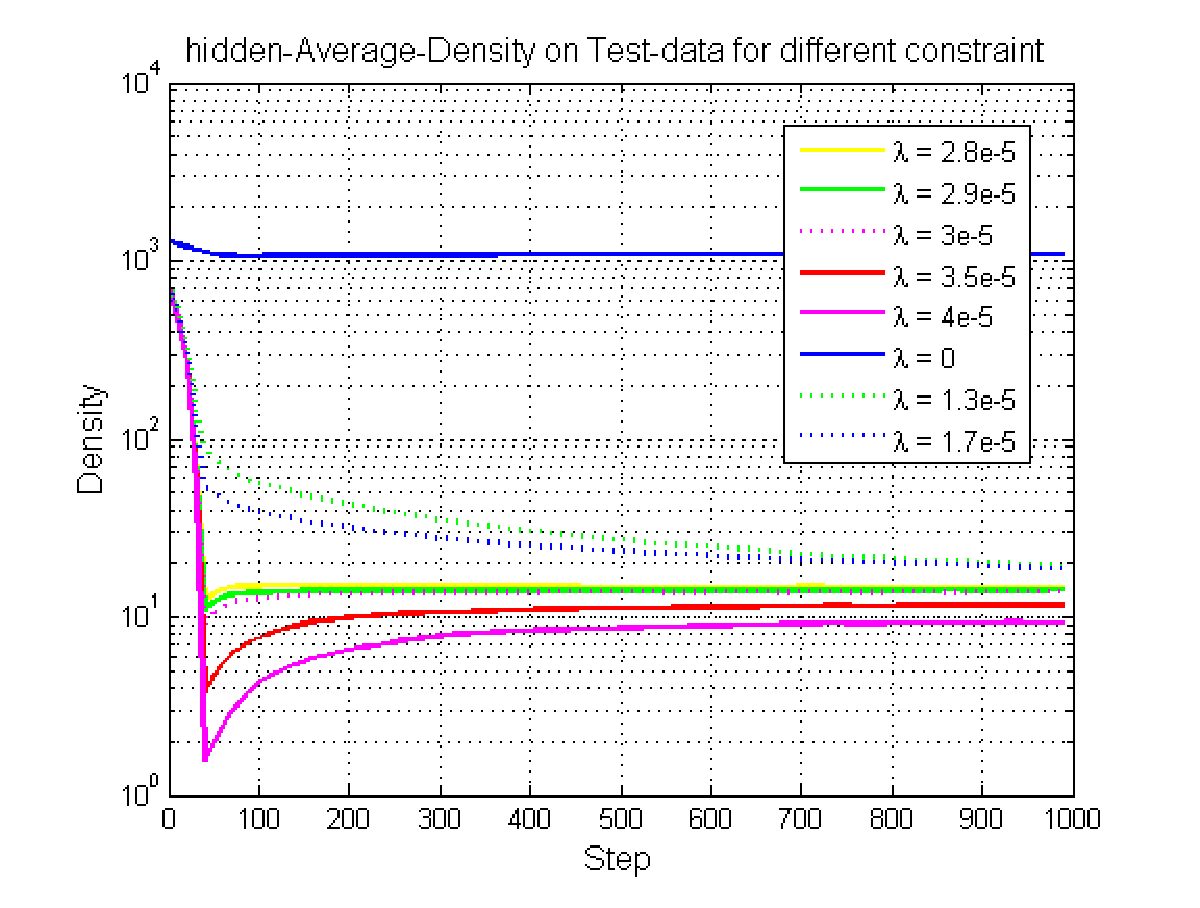
\includegraphics[width=4cm,height=3cm]{figure/hidden-Average-Density-on-Test-data-for-different-constraint_exp}
%\caption{Accuracy and Average-Density on test data for different-constraint.}
%\end{figure}

%\begin{figure}
%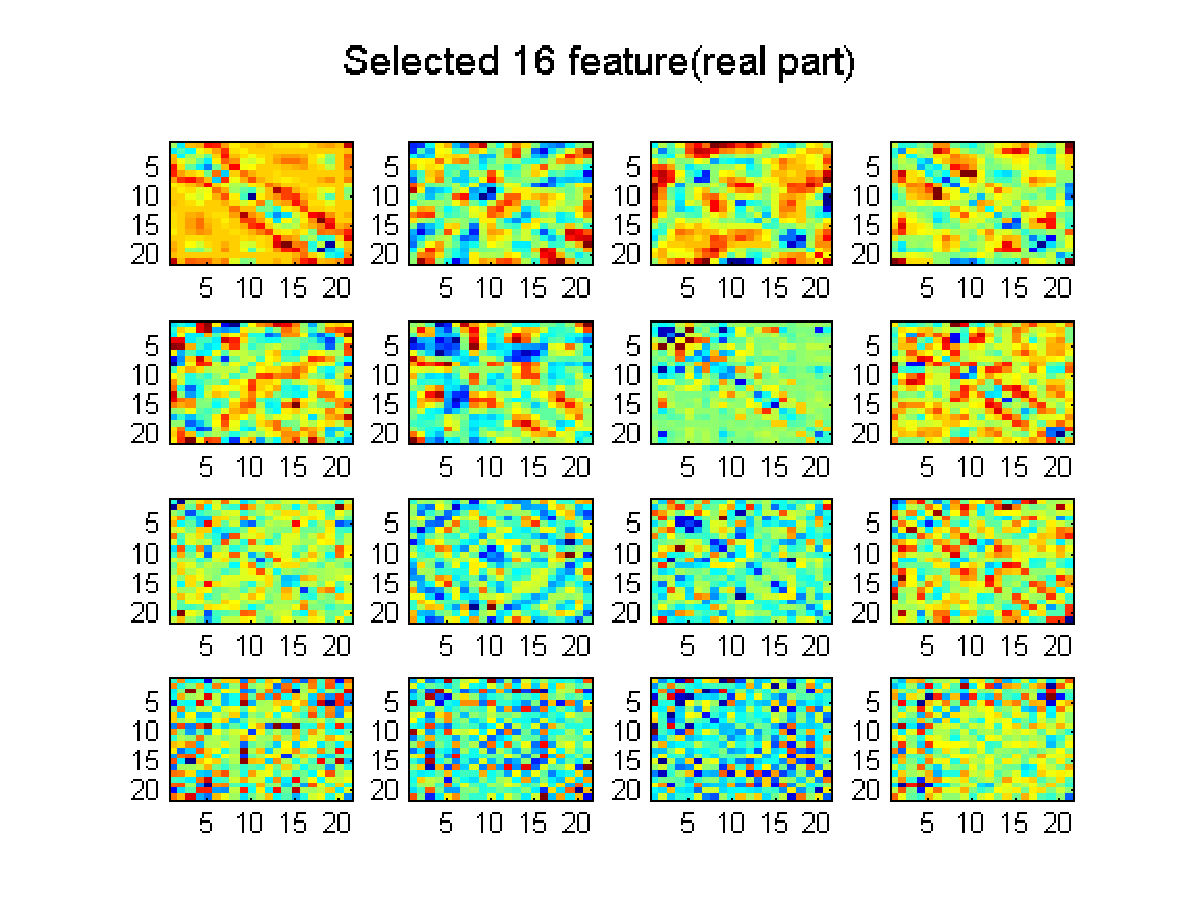
\includegraphics[width=4cm,height=3cm]{figure/selected_16_features_real_part}
%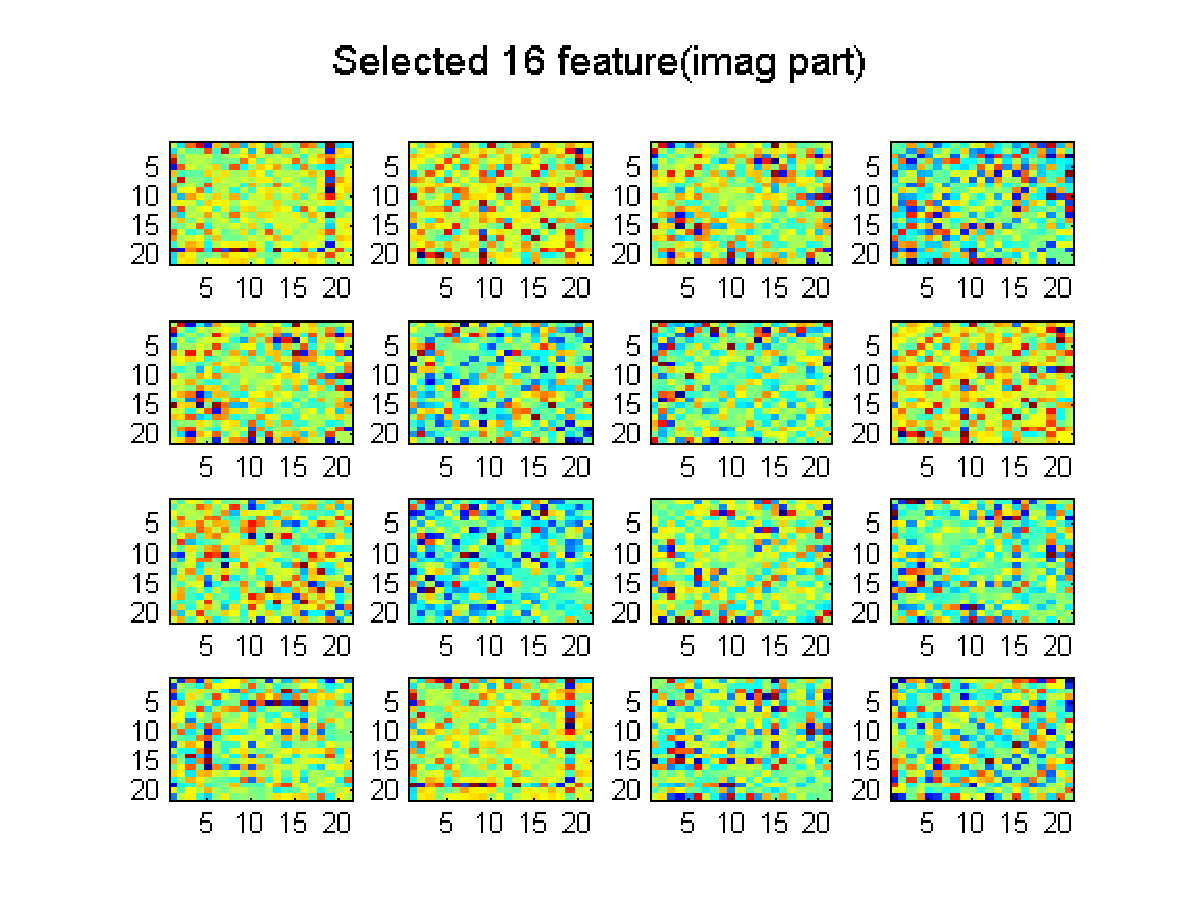
\includegraphics[width=4cm,height=3cm]{figure/selected_16_features_imag_part}
%\caption{Selected 16 features learned by neural network.}
%\end{figure}

\begin{figure}
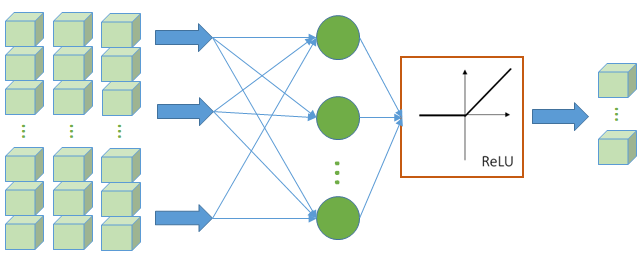
\includegraphics[width=8cm]{figure/sparse_represention_model}
\caption{The learned sparse representation model.The learned feature space spans data(scm) space likelihood that few basis functions $\phi$ explain a given data.}
\end{figure}

Apart from being beneficial to feature selection, sparse constraint can also reduce the activation rate of neurons in the hidden layer, without significant reduction in accuracy. In our example, when the coefficient is 2.1e-5, the average activation neuron number is just 16, which is greatly reduced, the activation rate is only 1.1{\%}.
These mean, in this example, the input 1323-elements SCM  data space can be represented by 740 feature vectors. Even more, averagely, each data sample can be represented by only 16 feature, as Fig.1 showns. The metadata is being compressed well. To sum up, by using regularization strategy on neural networks, we get a sparse and low rank model, where sparse means the transferred representation is sparse, low rank means the rank of learned weight matrix is low. The learned sparse coding model is Illustrated in Fig.3.
A sparse vector can be formed by filtering the data measured in sensor nodes through the pre-trained sparsely-coded neuron networks. Decisions, such as target location can be made by further processing.

\subsection{Comparison with conventional matched-field processing method}
As a comparison, here we use Bartlett Processor to position the source position, as Niu did in his work. There are two main kinds of replica-field used in Bartlett Processor, one is simulated by kraken(noted as bartlett 2), another is measurement data(noted as bartlett 1), same as the training data used in FNN.
% Please add the following required packages to your document preamble:
% \usepackage{booktabs}
\begin{table}[]
\caption{Localization accuracy of FNN and MFP on SWell96Ex-S5 data}
\label{my-label}
\begin{tabular}{@{}lllll@{}}
\toprule
Methods       & FNN    & MCE    & Bartlett 1 & Bartlett 2 \\ \midrule
109Hz         & 89.3\% & 72.3\% & 37.7\%     & 3.7\%      \\
232Hz         & 97\%   & 91\%   & 17.7\%     & 4.3\%      \\
385Hz         & 99.7\% & 97.7\% & 14\%       & 0.67\%     \\
109,232,385Hz & 99\%   & 99.7\% & 40.7\%     & 7.7\%      \\ \bottomrule
\end{tabular}
\end{table}

% Please add the following required packages to your document preamble:
% \usepackage{booktabs}
\begin{table}[]
\caption{Absolute mean error of FNN and MFP on SWell96Ex-S5 data(m)}
\label{my-label}
\begin{tabular}{@{}lllll@{}}
\toprule
Methods       & FNN  & MCE   & Bartlett 1 & Bartlett 2 \\ \midrule
109Hz         & 28.1 & 290.3 & 852.8      & 1219.5     \\
232Hz         & 7.4  & 2.5   & 832.3      & 832.3      \\
385Hz         & 0.08 & 0.58  & 1266.7     & 1756.3     \\
109,232,385Hz & 0.25 & 0.083 & 477.2      & 722.9      \\ \bottomrule
\end{tabular}
\end{table}

The accuracy and absolute mean error of different methods under different frequency are summed in table 1 and table 2. As we can see, whether it is in a single frequency or a mutli-frequency, the accuracy of FNN is always better than Bartlett, and not worse than direct data match(noted as MCE), which is more obvious when it come s to the comparison of absolute mean error. Thus, the study of neuron networks based sparse coding model is meaningful in positioning problem.

\subsection{The influences of ssp mismatch on FNN classifier}
In the MFP method, the model accuracy is heavily affected by the mismatch problem\cite{tolstoy1989sensitivity,feuillade1989environmental,del1988effects}. Fig.5 gives the FNN positioning results by simulations in different degrees change of sound speed profiles. Here, snapshot is 10 and SNR is 5dB.
Comparing to optimized-ssp, the i905-ssp has only a very small change, within 0.5m/s at the same depth. The change in i906-ssp is much significant, which can be seen from the shape in Fig.4.
\begin{figure}
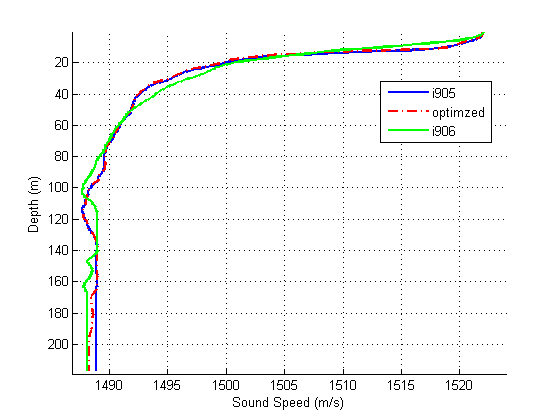
\includegraphics[width=6cm,height=5cm]{figure/ssp3}
\caption{Plots of sound speed profiles.}
\end{figure}

\begin{figure}
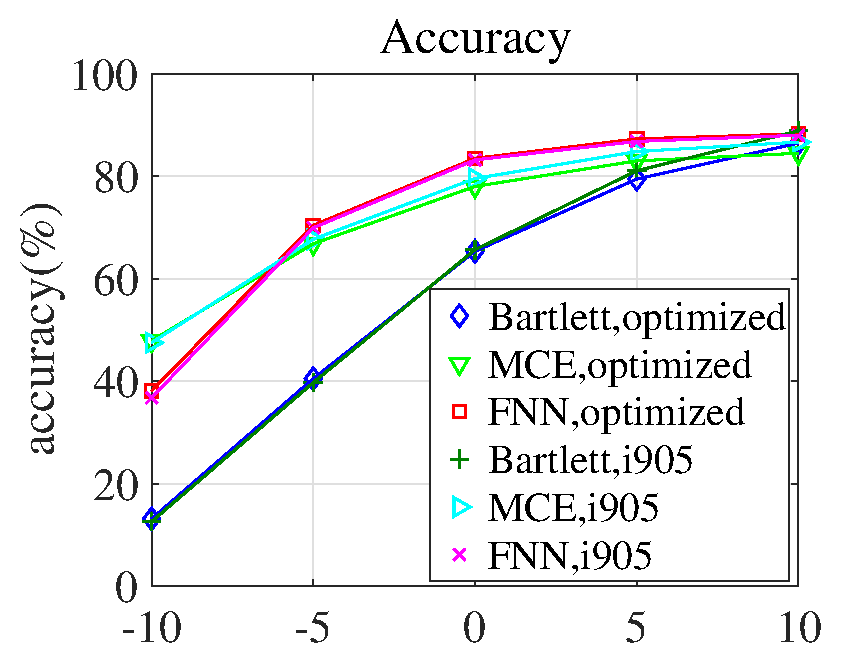
\includegraphics[width=4cm,height=3cm]{figure/Accuracy_to_SNR_FNN_vs_Bartlett_MCE}
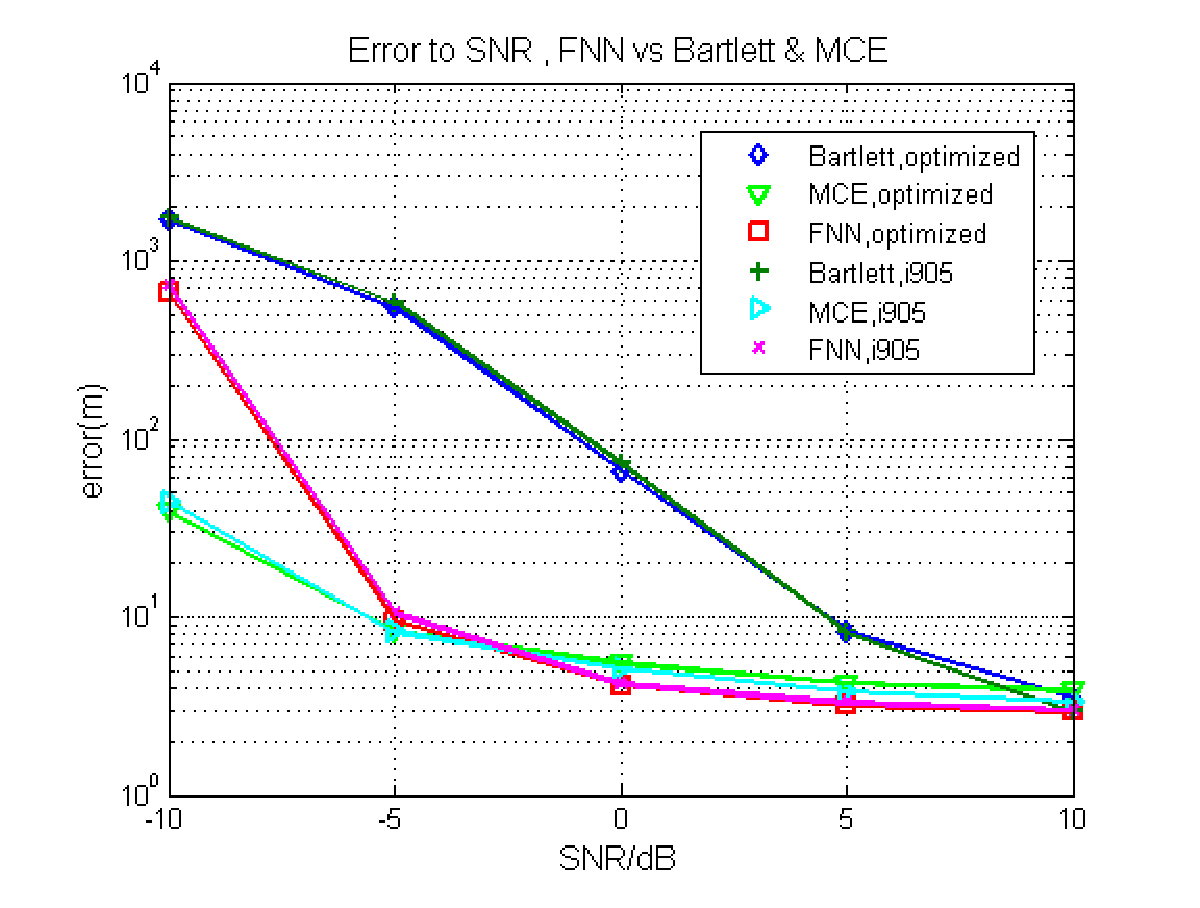
\includegraphics[width=4cm,height=3cm]{figure/Error_to_SNR_FNN_vs_Bartlett_MCE}
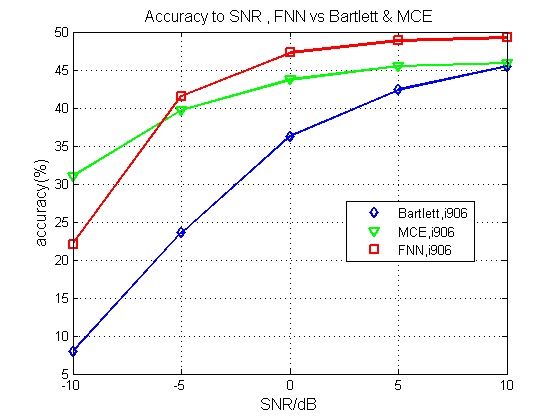
\includegraphics[width=4cm,height=3cm]{figure/Accuracy_to_SNR_FNN_vs_Bartlett_MCE_i906}
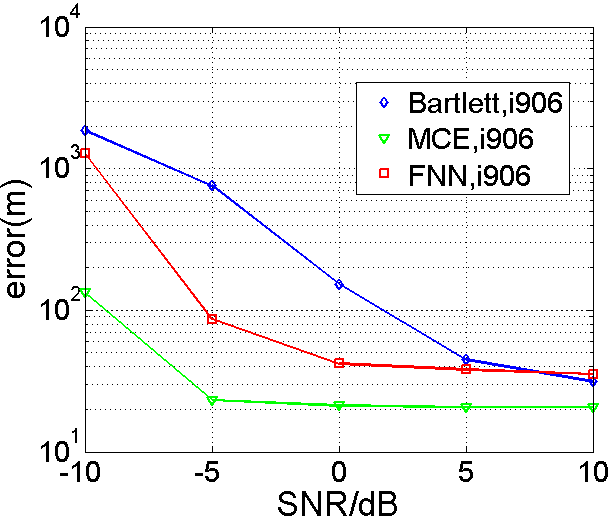
\includegraphics[width=4cm,height=3cm]{figure/Error_to_SNR_FNN_vs_Bartlett_MCE_i906}
\caption{FNN positioning performance curve on simulation data(frequency:109,232,385Hz).
 FNN is also sensitive to ssp mismatch, but still performs better than MFP.
}
\end{figure}

The performance curves for FNN, Bartlett, MCE is plotted by 1000 times Monte Carlo simulation. When the change in ssp is relatively small(the up two sub figures), FNN positioning best, MCE second and Bartlett worst.
When the shape of ssp change(the down two figures), the accuracy order unchanged, but the absolute error of FNN becomes bigger than MCE. FNN is also but less sensitive to ssp mismatch than Bartlett.

\begin{figure}
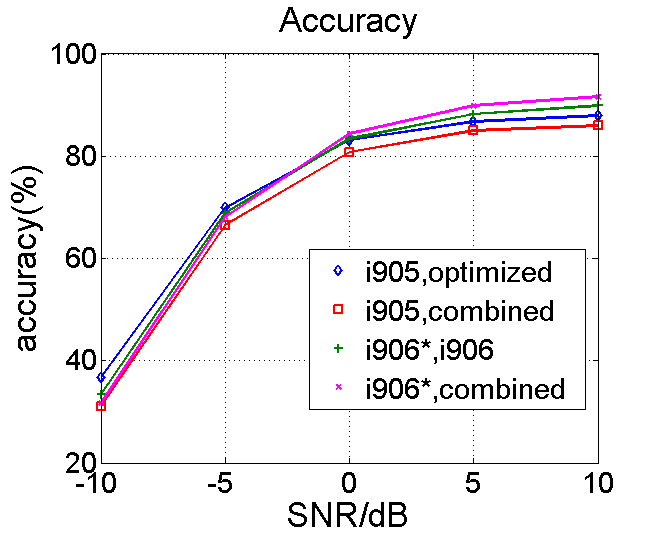
\includegraphics[width=4cm,height=3cm]{figure/Accuracy_to_SNR_Combined_vs_Single}
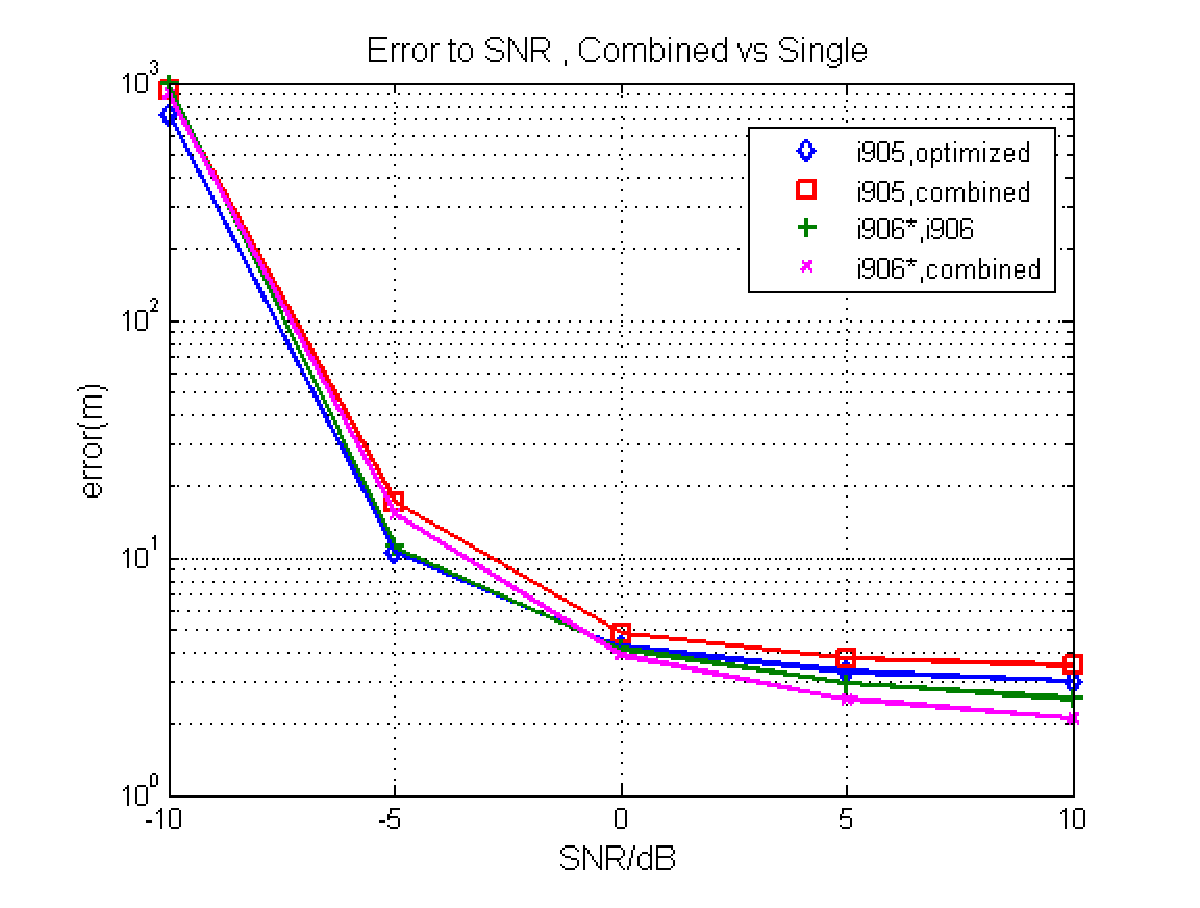
\includegraphics[width=4cm,height=3cm]{figure/Error_to_SNR_Combined_vs_Single}
\caption{FNN positioning performance curve on simulation data. FNN model tolerance can be by significantly improved by mixed data training}
\end{figure}

\subsection{%Co-training using data collected from different ssp
Increase model tolerance by data-model mixed training}
The simulation results show that training the model using data collected from different ssp can significantly improve the tolerance of the classifier, which means FNN can learn weights over a set of changing ssp.

%\begin{figure}
%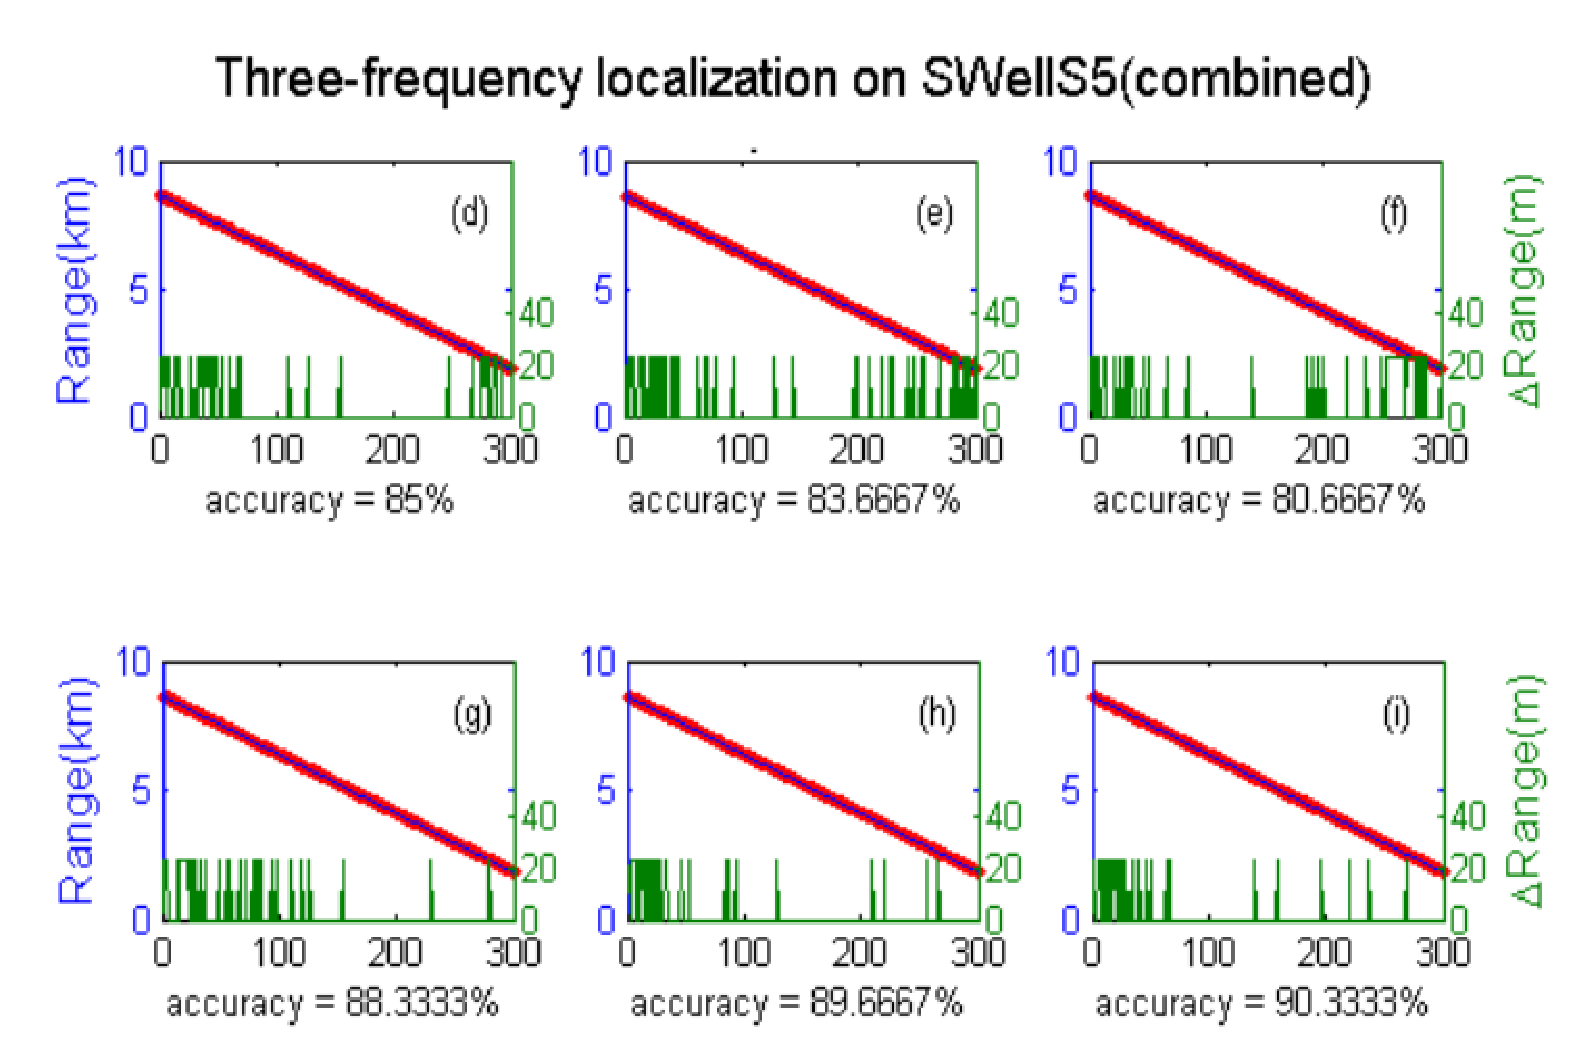
\includegraphics[width=4cm,height=3cm]{figure/combinevssingle_lef}
%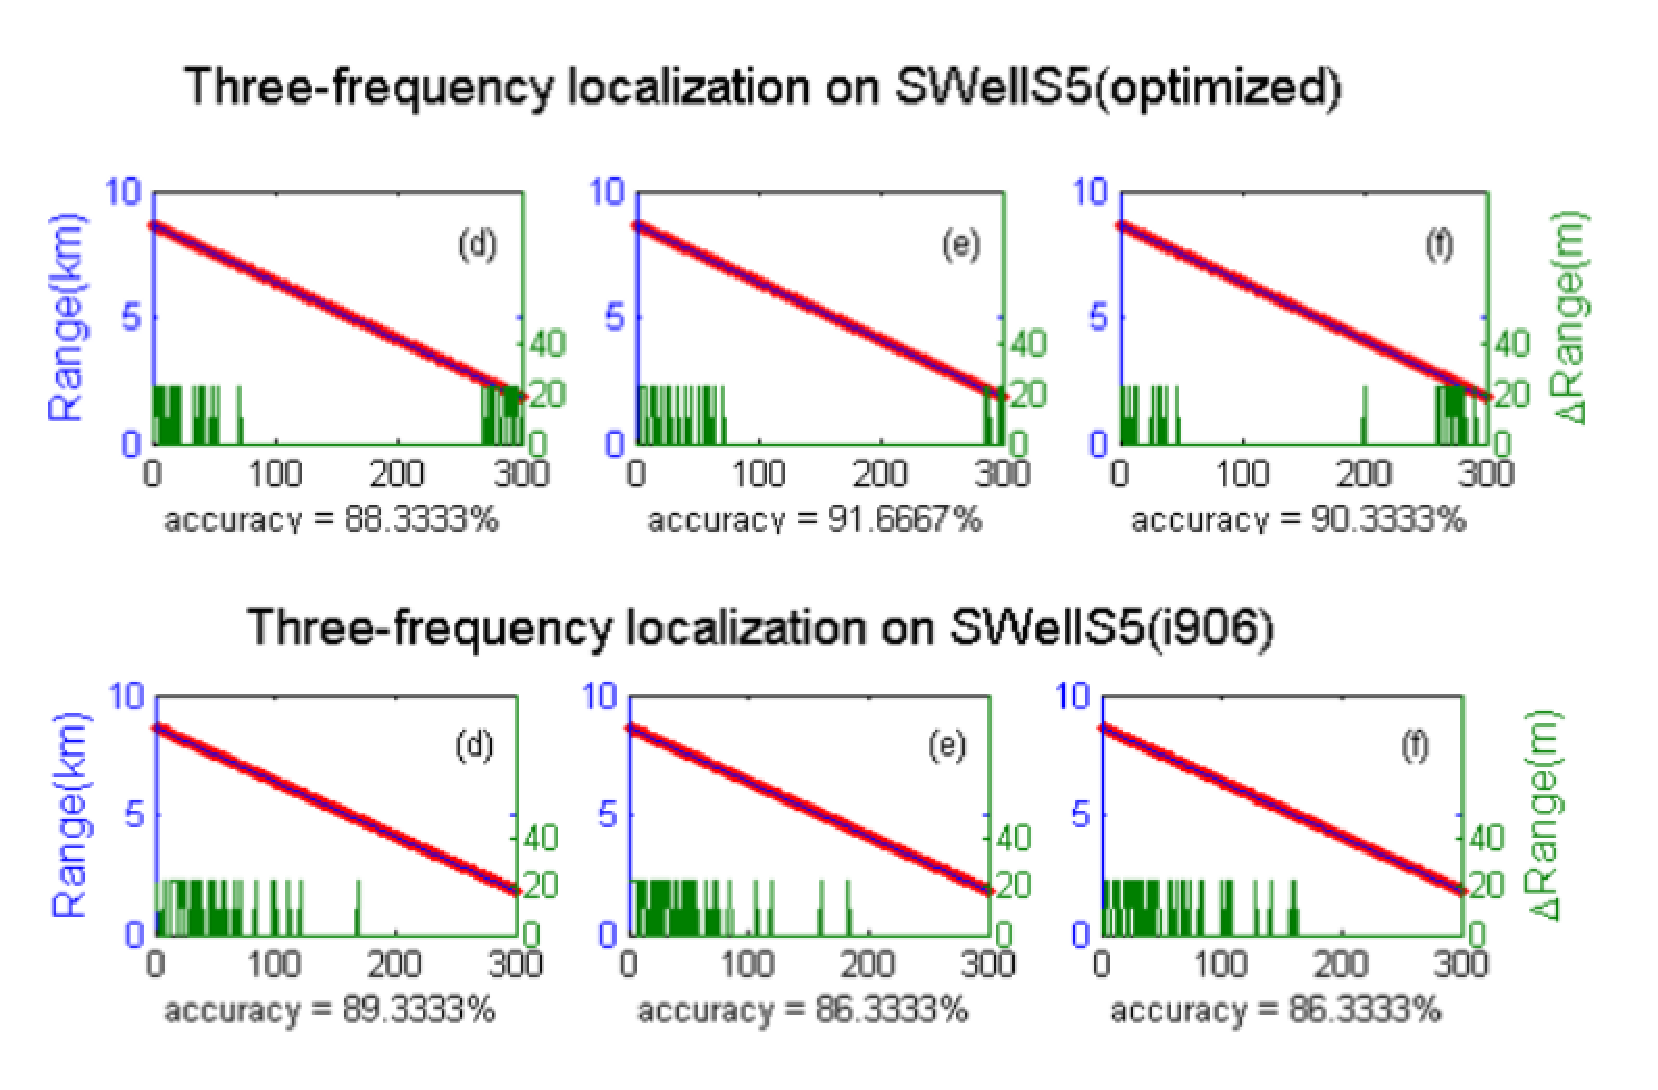
\includegraphics[width=4cm,height=3cm]{figure/combinevssingle_right}
%\caption{Comparison of mixed data training and single data training .}
%\end{figure}

As discussed in section 3.4, the FNN is also sensitive to ssp mismatch, but still performs better than Bartlett. When the environment ssp has a big change in the shape(such as from ssp-optimized to i906), the performance of the estimator drops about 40\% in accuracy. In this section, by adding some data collected from i906-ssp, the positioning ability of FNN on i906{*}(which is little changed from i906,for the sake of testing) is as better as before. Although the accuracy for i905 has a little glissade compared with single data training case, the performance for i906 improved. In general, the trained FNN classifier works well on both two different shape ssp. Note that, the legend 'i905,combined' means the model is trained by mixed data collected from ssp i906 and ssp optimized, then the model is tested on ssp i905, rests is similar.

\section{Conclusions}
%In a recent article\cite{niu2017source}, Niu considers the problem of sound source location in marine waveguides as a classification problem under the framework of machine learning,and verified the ideal on the Noise09 experimental data.
%Due to the requirement for energy and computations, it is essential to develop methods to effectively exact specific task-relevant information from measures.
It is attractive to see that neural networks trained with sparse constraint learns a set of features with specific structures and can help construct a sparsely-coded neural network, which reduce the number of features needed to explain a given measured data. Comparing with conventional matched-feld processing method, the neural network model performs better in mismatch cases, and it's tolerance can be obviously increased by data-model mixed training. It deserves more effort to apply more machine learning models on ocean acoustic source localization. 

\begin{acks}
The work is supported by ...

\end{acks}
